\documentclass{ximera}

%\usepackage{todonotes}

\newcommand{\todo}{}


\graphicspath{
{./}
{../functionsOfSeveralVariables/}
{../normalVectors/}
{../lagrangeMultipliers/}
}


\usepackage{tkz-euclide}
\tikzset{>=stealth} %% cool arrow head
\tikzset{shorten <>/.style={ shorten >=#1, shorten <=#1 } } %% allows shorter vectors

\usetikzlibrary{backgrounds} %% for boxes around graphs
\usetikzlibrary{shapes,positioning}  %% Clouds and stars
\usetikzlibrary{matrix} %% for matrix
\usepgfplotslibrary{polar} %% for polar plots
\usetkzobj{all}
\usepackage[makeroom]{cancel} %% for strike outs
%\usepackage{mathtools} %% for pretty underbrace % Breaks Ximera
\usepackage{multicol}





\usepackage{array}
\setlength{\extrarowheight}{+.1cm}   
\newdimen\digitwidth
\settowidth\digitwidth{9}
\def\divrule#1#2{
\noalign{\moveright#1\digitwidth
\vbox{\hrule width#2\digitwidth}}}





\newcommand{\RR}{\mathbb R}
\newcommand{\R}{\mathbb R}
\newcommand{\N}{\mathbb N}
\newcommand{\Z}{\mathbb Z}

\newcommand{\sage}{\textsf{SageMath}}


%\renewcommand{\d}{\,d\!}
\renewcommand{\d}{\mathop{}\!d}
\newcommand{\dd}[2][]{\frac{\d #1}{\d #2}}
\newcommand{\pp}[2][]{\frac{\partial #1}{\partial #2}}
\renewcommand{\l}{\ell}
\newcommand{\ddx}{\frac{d}{\d x}}

\newcommand{\zeroOverZero}{\ensuremath{\boldsymbol{\tfrac{0}{0}}}}
\newcommand{\inftyOverInfty}{\ensuremath{\boldsymbol{\tfrac{\infty}{\infty}}}}
\newcommand{\zeroOverInfty}{\ensuremath{\boldsymbol{\tfrac{0}{\infty}}}}
\newcommand{\zeroTimesInfty}{\ensuremath{\small\boldsymbol{0\cdot \infty}}}
\newcommand{\inftyMinusInfty}{\ensuremath{\small\boldsymbol{\infty - \infty}}}
\newcommand{\oneToInfty}{\ensuremath{\boldsymbol{1^\infty}}}
\newcommand{\zeroToZero}{\ensuremath{\boldsymbol{0^0}}}
\newcommand{\inftyToZero}{\ensuremath{\boldsymbol{\infty^0}}}



\newcommand{\numOverZero}{\ensuremath{\boldsymbol{\tfrac{\#}{0}}}}
\newcommand{\dfn}{\textbf}
%\newcommand{\unit}{\,\mathrm}
\newcommand{\unit}{\mathop{}\!\mathrm}
\newcommand{\eval}[1]{\bigg[ #1 \bigg]}
\newcommand{\seq}[1]{\left( #1 \right)}
\renewcommand{\epsilon}{\varepsilon}
\renewcommand{\iff}{\Leftrightarrow}

\DeclareMathOperator{\arccot}{arccot}
\DeclareMathOperator{\arcsec}{arcsec}
\DeclareMathOperator{\arccsc}{arccsc}
\DeclareMathOperator{\si}{Si}
\DeclareMathOperator{\proj}{\vec{proj}}
\DeclareMathOperator{\scal}{scal}
\DeclareMathOperator{\sign}{sign}


%% \newcommand{\tightoverset}[2]{% for arrow vec
%%   \mathop{#2}\limits^{\vbox to -.5ex{\kern-0.75ex\hbox{$#1$}\vss}}}
\newcommand{\arrowvec}{\overrightarrow}
%\renewcommand{\vec}[1]{\arrowvec{\mathbf{#1}}}
\renewcommand{\vec}{\mathbf}
\newcommand{\veci}{{\boldsymbol{\hat{\imath}}}}
\newcommand{\vecj}{{\boldsymbol{\hat{\jmath}}}}
\newcommand{\veck}{{\boldsymbol{\hat{k}}}}
\newcommand{\vecl}{\boldsymbol{\l}}
\newcommand{\utan}{\mathbf{\hat{t}}}
\newcommand{\unormal}{\mathbf{\hat{n}}}
\newcommand{\ubinormal}{\mathbf{\hat{b}}}

\newcommand{\dotp}{\bullet}
\newcommand{\cross}{\boldsymbol\times}
\newcommand{\grad}{\boldsymbol\nabla}
\newcommand{\divergence}{\grad\dotp}
\newcommand{\curl}{\grad\cross}
%\DeclareMathOperator{\divergence}{divergence}
%\DeclareMathOperator{\curl}[1]{\grad\cross #1}
\newcommand{\lto}{\mathop{\longrightarrow\,}\limits}


\colorlet{textColor}{black} 
\colorlet{background}{white}
\colorlet{penColor}{blue!50!black} % Color of a curve in a plot
\colorlet{penColor2}{red!50!black}% Color of a curve in a plot
\colorlet{penColor3}{red!50!blue} % Color of a curve in a plot
\colorlet{penColor4}{green!50!black} % Color of a curve in a plot
\colorlet{penColor5}{orange!80!black} % Color of a curve in a plot
\colorlet{fill1}{penColor!20} % Color of fill in a plot
\colorlet{fill2}{penColor2!20} % Color of fill in a plot
\colorlet{fillp}{fill1} % Color of positive area
\colorlet{filln}{penColor2!20} % Color of negative area
\colorlet{fill3}{penColor3!20} % Fill
\colorlet{fill4}{penColor4!20} % Fill
\colorlet{fill5}{penColor5!20} % Fill
\colorlet{gridColor}{gray!50} % Color of grid in a plot

\newcommand{\surfaceColor}{violet}
\newcommand{\surfaceColorTwo}{redyellow}
\newcommand{\sliceColor}{greenyellow}




\pgfmathdeclarefunction{gauss}{2}{% gives gaussian
  \pgfmathparse{1/(#2*sqrt(2*pi))*exp(-((x-#1)^2)/(2*#2^2))}%
}


%%%%%%%%%%%%%
%% Vectors
%%%%%%%%%%%%%

%% Simple horiz vectors
\renewcommand{\vector}[1]{\left\langle #1\right\rangle}


%% %% Complex Horiz Vectors with angle brackets
%% \makeatletter
%% \renewcommand{\vector}[2][ , ]{\left\langle%
%%   \def\nextitem{\def\nextitem{#1}}%
%%   \@for \el:=#2\do{\nextitem\el}\right\rangle%
%% }
%% \makeatother

%% %% Vertical Vectors
%% \def\vector#1{\begin{bmatrix}\vecListA#1,,\end{bmatrix}}
%% \def\vecListA#1,{\if,#1,\else #1\cr \expandafter \vecListA \fi}

%%%%%%%%%%%%%
%% End of vectors
%%%%%%%%%%%%%

%\newcommand{\fullwidth}{}
%\newcommand{\normalwidth}{}



%% makes a snazzy t-chart for evaluating functions
%\newenvironment{tchart}{\rowcolors{2}{}{background!90!textColor}\array}{\endarray}

%%This is to help with formatting on future title pages.
\newenvironment{sectionOutcomes}{}{} 



%% Flowchart stuff
%\tikzstyle{startstop} = [rectangle, rounded corners, minimum width=3cm, minimum height=1cm,text centered, draw=black]
%\tikzstyle{question} = [rectangle, minimum width=3cm, minimum height=1cm, text centered, draw=black]
%\tikzstyle{decision} = [trapezium, trapezium left angle=70, trapezium right angle=110, minimum width=3cm, minimum height=1cm, text centered, draw=black]
%\tikzstyle{question} = [rectangle, rounded corners, minimum width=3cm, minimum height=1cm,text centered, draw=black]
%\tikzstyle{process} = [rectangle, minimum width=3cm, minimum height=1cm, text centered, draw=black]
%\tikzstyle{decision} = [trapezium, trapezium left angle=70, trapezium right angle=110, minimum width=3cm, minimum height=1cm, text centered, draw=black]


\title[Dig-In:]{Parametric surfaces}

\begin{document}
\begin{abstract}
  Tangent and normal vectors can help model surfaces in space.
\end{abstract}
\maketitle


\section{Thickening a curve}

Suppose you have been a curve in space, and you want to build a
parameterized surface which is a ``thickened'' version.  In other
words, we want to convert a curve like
\begin{image}
  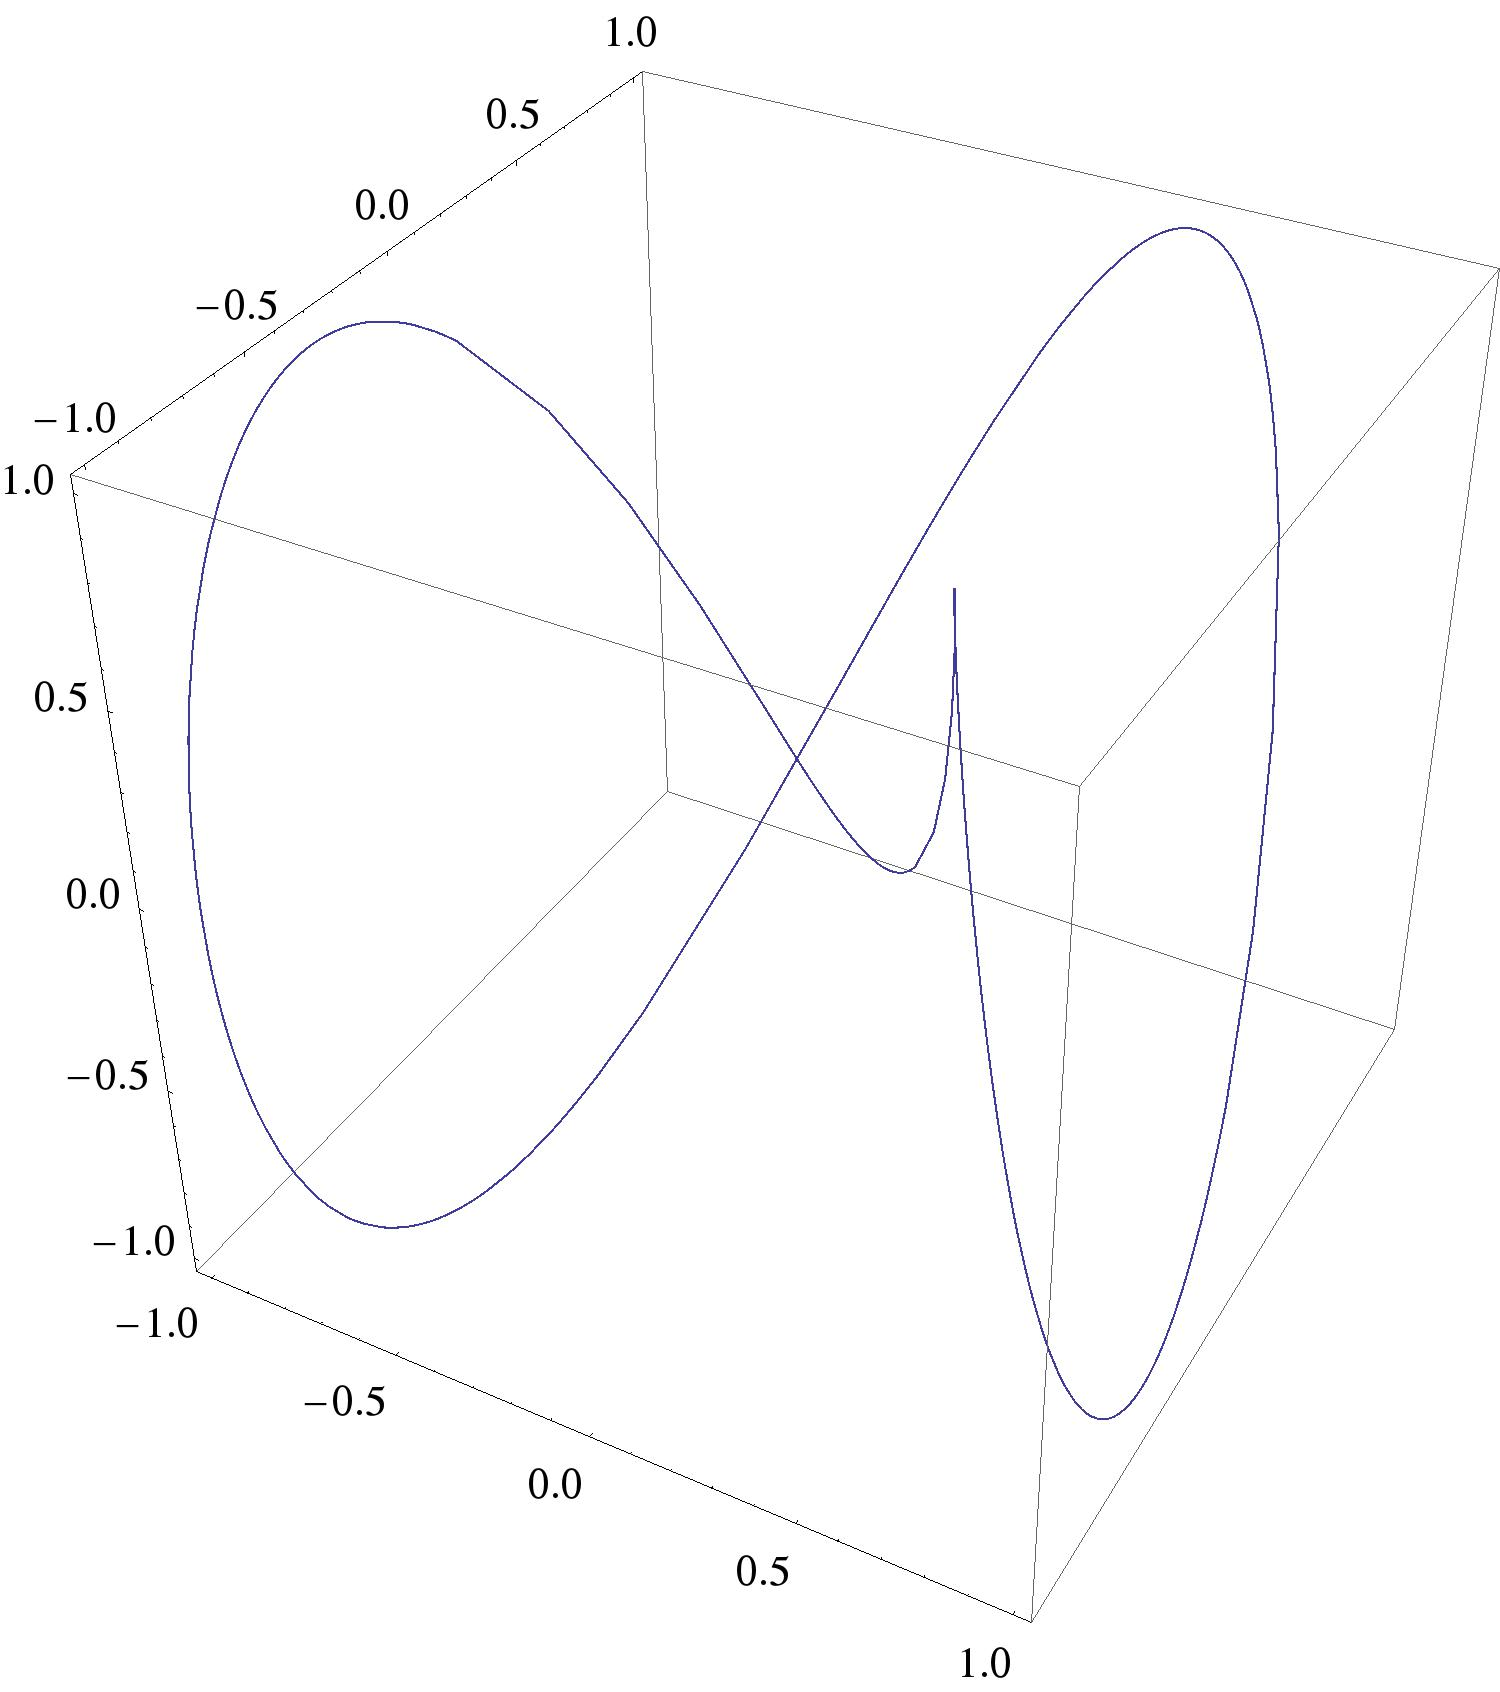
\includegraphics{curve.jpg}
\end{image}
%% \begin{sageOutput}
%% x(t) = sin(t)
%% y(t) = sin(2*t + pi/5)
%% z(t) = sin(3*t + pi/7)
%% f(t) = (x(t),y(t),z(t))
%% parametric_plot3d(f(t), (t,0,2*pi))
%%   \end{sageOutput}
into a thickened ``tube'' like
\begin{image}
  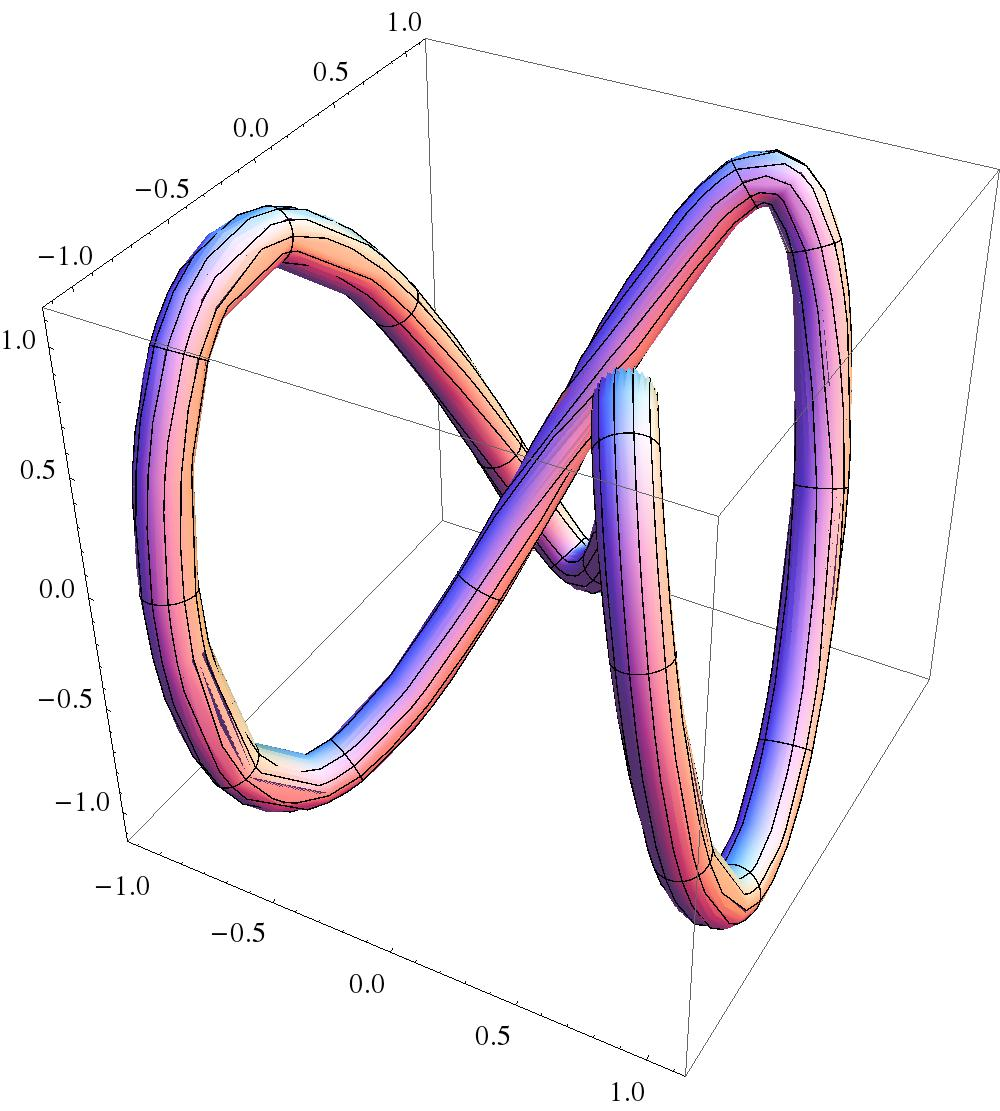
\includegraphics{tube.jpg}
\end{image}
%% \begin{sageOutput}
%% var('s')
%% x(t) = sin(t)
%% y(t) = sin(2*t + pi/5)
%% z(t) = sin(3*t + pi/7)
%% f(t) = (x(t),y(t),z(t))
%% df=derivative(f,t)
%% ut = df / df.norm()
%% ddf = derivative(ut,t)
%% n = ddf / ddf.norm()
%% bn = n.cross_product(ut)
%% thickness = 0.10
%% parametric_plot3d(f(t) + (n * cos(s) + bn * sin(s)) * thickness, (t,0,2*pi), (s,0,2*pi), plot_points=[100,100])
%%   \end{sageOutput}
%% \begin{image}
%%   \begin{tikzpicture}
%%     \begin{axis}[tick label style={font=\scriptsize},axis on top,view={-30}{30},no markers,zmax=1,axis lines=center,
%%         ymax=1.5,ymin=-1.5,clip=false,
%%         xmax=1.5,xmin=-1.5,
%%         every axis x label/.style={at={(axis cs:\pgfkeysvalueof{/pgfplots/xmax},0,0)},xshift=-3pt,yshift=-3pt},
%% 	xlabel={\scriptsize $x$},
%% 	every axis y label/.style={at={(axis cs:0,\pgfkeysvalueof{/pgfplots/ymax},0)},xshift=0pt,yshift=-5pt},
%% 	ylabel={\scriptsize $y$},
%% 	every axis z label/.style={at={(axis cs:0,0,\pgfkeysvalueof{/pgfplots/zmax})},xshift=0pt,yshift=4pt},
%% 	zlabel={\scriptsize $z$}]
%%       \addplot3+[domain=-0:360,samples=200,samples y=0,ultra thick](sin(x),{sin(2*x+36},{sin(3*x+25)});
%%     \end{axis}
%%   \end{tikzpicture}
%% \end{image}

\begin{example}
  You have been given a curve in space, say
  \[
  \vec{f}(t) = \langle t^2-2, t^2-2, 1-t\rangle.
  \]
  We want to make a tube around it of radius $0.5$.
  \begin{explanation}
    Here is the idea, we want to take our curve and attach two
    orthogonal vectors to every point
    \begin{image}
      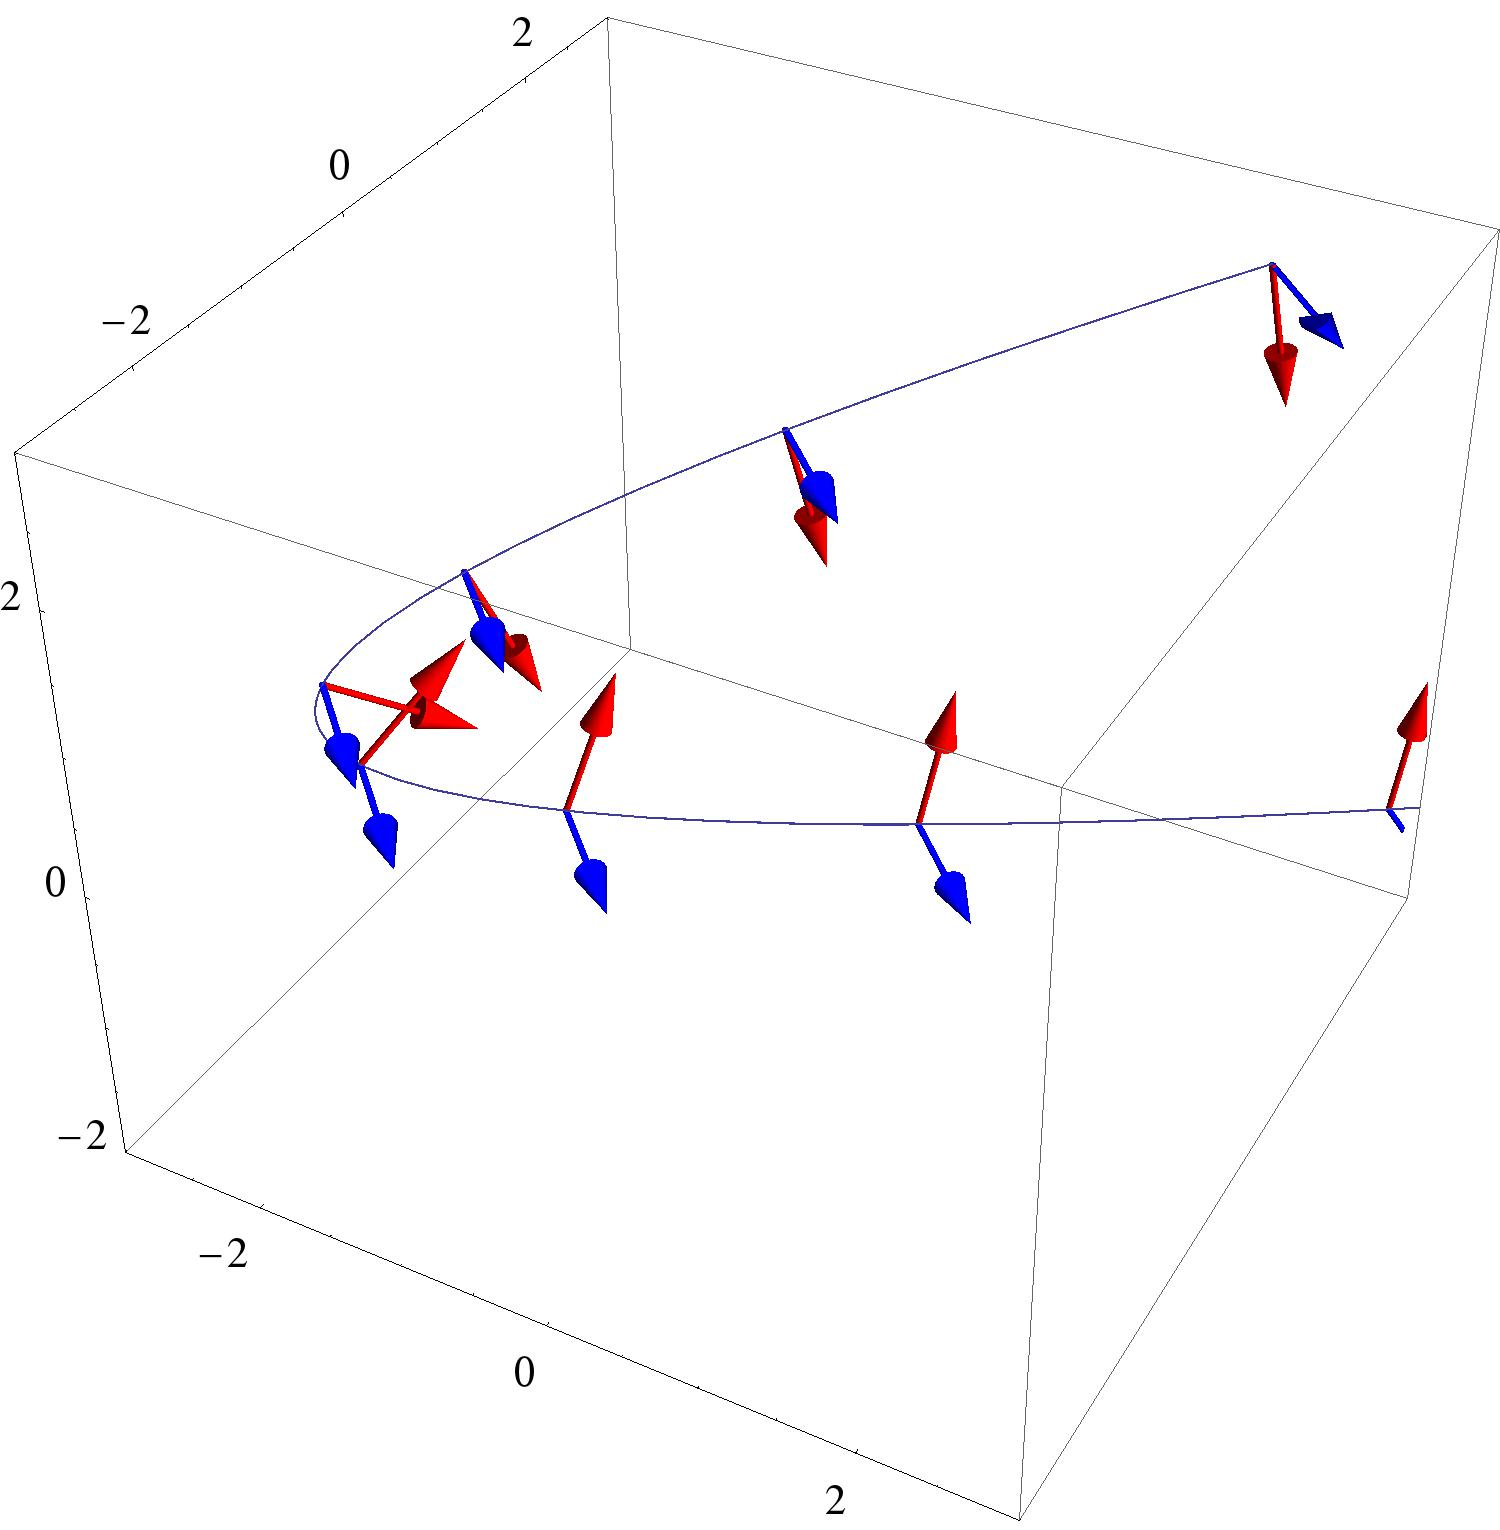
\includegraphics{paraArrows.jpg}
    \end{image}
    We'll start by computing the
    \wordChoice{\choice[correct]{unit tangent}\choice{unit normal}\choice{unit binormal}}
    vectors. Write with me
    \[
    \utan(t) = \frac{\vec{f}'(t)}{|\vec{f}'(t)|}
    \]
    From these vectors we can obtain the \wordChoice{\choice{unit
        tangent}\choice[correct]{unit normal}\choice{unit binormal}}
    vectors by differentiating:
    \[
    \unormal(t) = \frac{\utan'(t)}{|\utan'(t)|}
    \]
    Finally we can obtain the \wordChoice{\choice{unit
        tangent}\choice{unit normal}\choice[correct]{unit binormal}}
    vectors via the cross product:
    \[
    \ubinormal(t) = \utan(t) \cross \unormal(t)
    \]
    Looking again at
    \begin{image}
      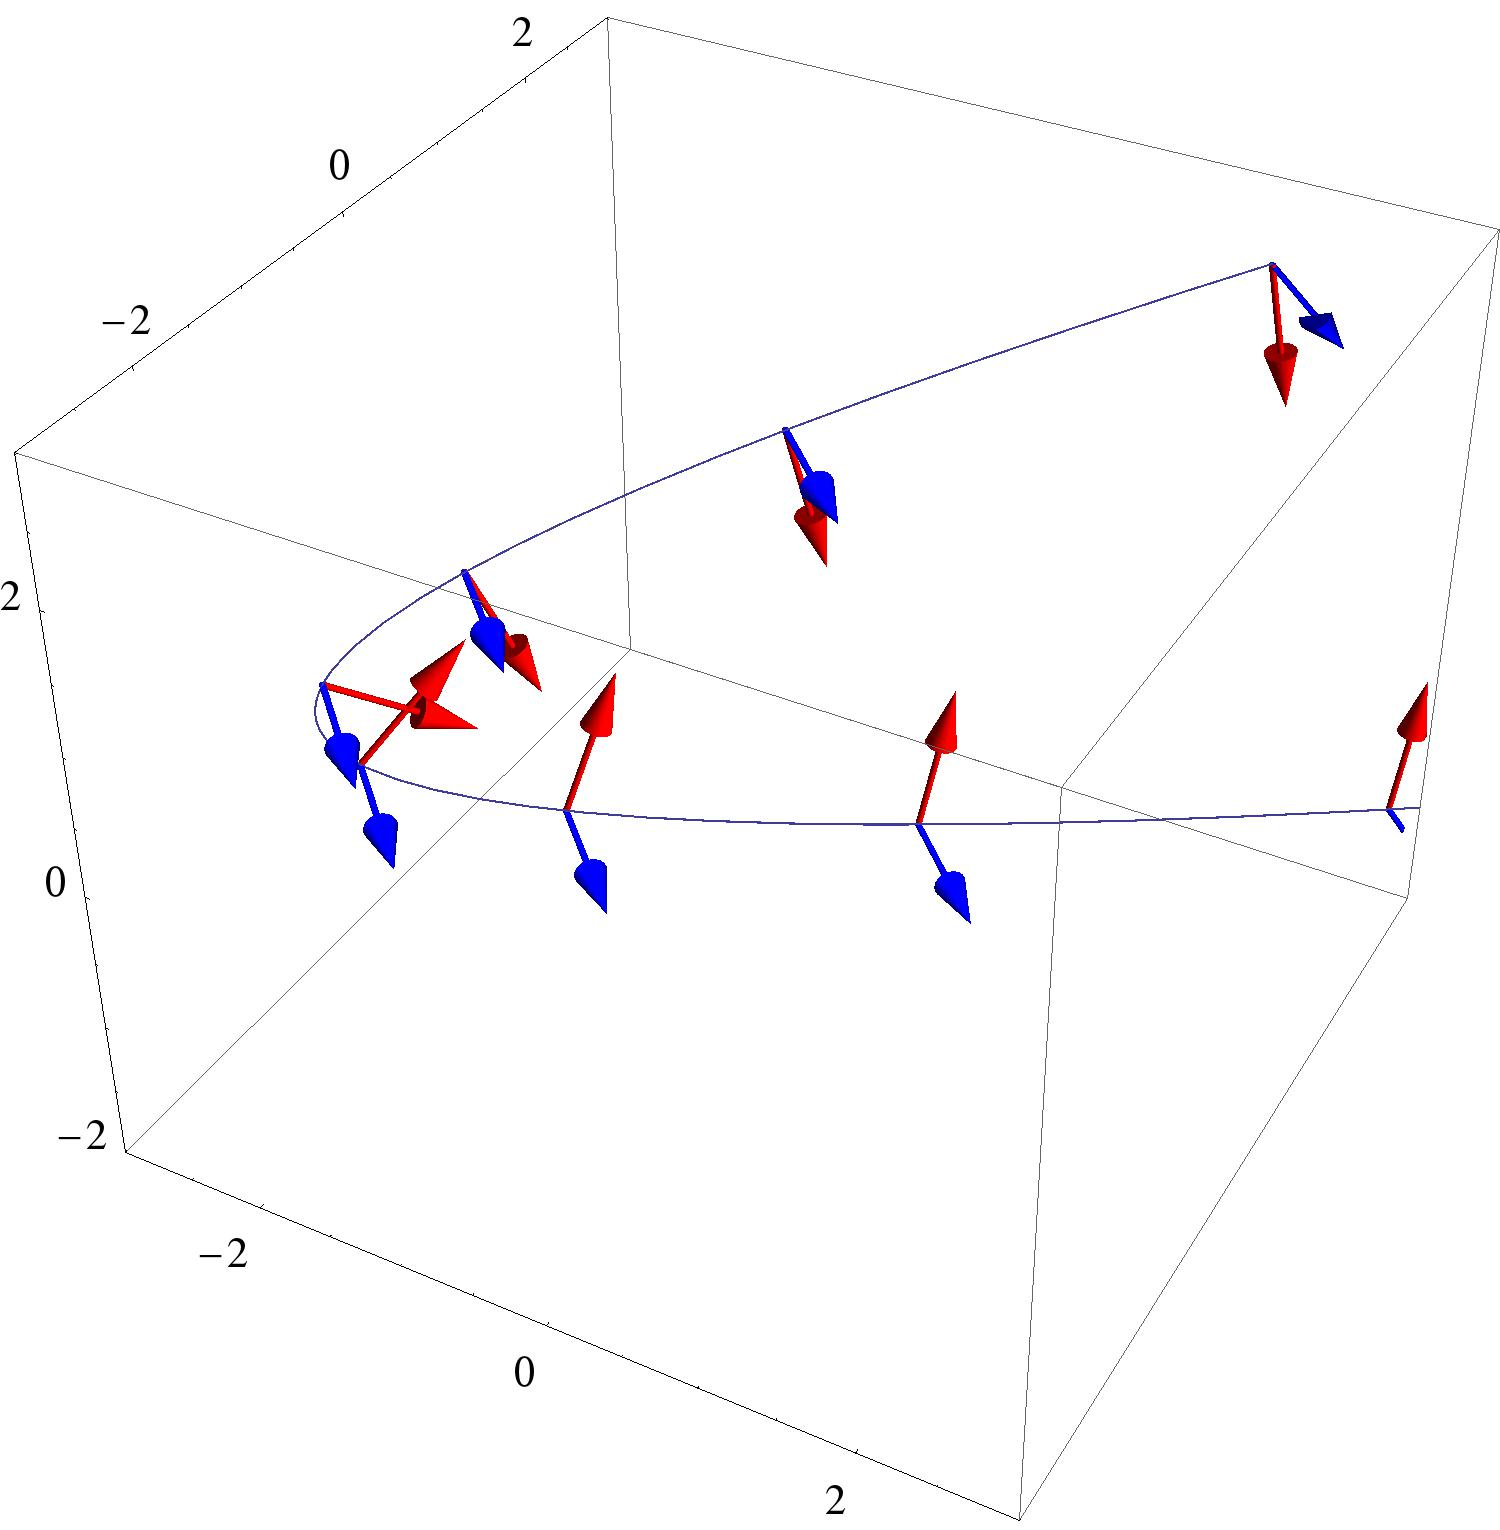
\includegraphics{paraArrows.jpg}
    \end{image}
    we see the unit normal vectors in red, and the unit binormal
    vectors in blue. So we now can plot our tube:
    \[
    \vec{F}(s,t) = \vec{f}(t) + 0.5 \unormal(t)\cos(s) + 0.5 \ubinormal(t)\sin(s)
    \]
    \begin{onlineOnly}
      We can check our work with \sage.
  \begin{sageCell}
var('s t')
x(t) = t^2-2
y(t) = t^2-2
z(t) = 1-t
f(t) = (x(t),y(t),z(t))
df=derivative(f,t)
ut = df / df.norm()
ddf = derivative(ut,t)
n = ddf / ddf.norm()
bn = ut.cross_product(n)
parametric_plot3d(f(t) + 0.5*n*cos(s) + 0.5*bn*sin(s), (t,-3,3), (s,0,2*pi))
  \end{sageCell}
    \end{onlineOnly}
  \end{explanation}
\end{example}



  Our tube around $\vec{f}$ will be a parametrized surface given by 
  \begin{multipleChoice}
    \choice{$\vec{f}: \R \to \R^2$}
    \choice{$F: \R^2 \to \R$}
    \choice[correct]{$\vec{F}: \R^2 \to \R^3$}
    \choice{$\vec{F}: \R^3 \to \R^2$}
  \end{multipleChoice}

  We can parametrize a circle with
  \begin{multipleChoice}
    \choice{$t \mapsto (x^2, y^2)$}
    \choice{$t \mapsto (\cos^2(t), \sin^2(t))$}
    \choice[correct]{$t \mapsto (\cos(t), \sin(t))$}
  \end{multipleChoice}
  so we \textit{could} try
  \[
    \vec{F}(t,s) = \vec{f}(t) + 0.25 \vector{\cos s, \sin s, 0}.
  \]
  Note that we are using \textbf{vector operations}---we are taking the
\wordChoice{\choice[correct]{sum}\choice{dot product}} of two vectors to build up our parametrized surface.  We want the vector $\vec{f}(t)$ to sit \wordChoice{\choice{on the surface}\choice[correct]{inside the tube}} and the second term pushes us away from $\vec{f}(t)$ in a different direction as $s$ varies.  The factor of 0.25 is included to \wordChoice{\choice[correct]{shrink the circle}\choice{expand the circle}}.  Putting this together, we can see a picture emerging:
  \begin{sageCell}
t = var('t')
x = sin(t) ; y = sin(2*t + pi/5) ; z = sin(3*t + pi/7)
f = vector([x,y,z])

s = var('s')
parametric_plot3d( f + 0.25 * vector([cos(s), sin(s), 0]), (t,0,2*pi), (s,0,2*pi) )
\end{sageCell}
and that doesn't look awful, but it also certainly doesn't quite look
right!  The trouble is the circle we sweep out with
$\vector{\cos s, \sin s, 0}$ is not always
\wordChoice{\choice[correct]{perpendicular}\choice{parallel}} to the
unit tangent vector, defined as
\begin{multipleChoice}
  \choice{$\utan(t) = \frac{\vec{f}'(t)}{|\vec{f}'(t)|^2}$}
  \choice[correct]{$\utan(t) = \frac{\vec{f}'(t)}{|\vec{f}'(t)|}$}
\end{multipleChoice}
To improve our tube, we want to sweep out a circle in the plane given by
\begin{multipleChoice}
  \choice{$\utan(t)$ and $\unormal(t)$}
  \choice{$\utan(t)$ and $\unormal(t) \cross \utan(t)$}
  \choice[correct]{$\unormal(t)$ and $\unormal(t) \cross \utan(t)$}
\end{multipleChoice}
Let $\vec{b} = \unormal(t) \cross \utan(t)$ and $\ubinormal = \frac{\vec{b}}{| \vec{b} |}$.  Then we can sweep out a tube with
  \[
    \vec{F}(t,s) = \vec{f}(t) + 0.25 \left( \left( \cos \answer{s} \right) \unormal(\answer{t}) + \left( \sin s \right) \ubinormal(t) \right)
  \]
  to keep our circle in the appropriate plane.  Try it!
\begin{sageCell}
t = var('t')
x = sin(t) ; y = sin(2*t + pi/5) ; z = sin(3*t + pi/7)

f = vector([x,y,z])
df = derivative(f,t)
u = df.normalized()
n = derivative(u,t).normalized()
b = n.cross_product(u).normalized()

thickness = 0.25
s = var('s')
parametric_plot3d( f + (n * cos(s) + b * sin(s)) * thickness, (t,0,2*pi), (s,0,2*pi), plot_points=[100,100] )
\end{sageCell}


\begin{example}[Mirrored surfaces]
  We have a parametrized surface 
  \begin{multipleChoice}
    \choice{$\vec{f}: \R \to \R^2$}
    \choice{$F: \R^2 \to \R$}
    \choice[correct]{$\vec{F}: \R^2 \to \R^3$}
    \choice{$\vec{F}: \R^3 \to \R^2$}
  \end{multipleChoice}
  given by $(a,b) \mapsto (a, b, a^2 + b^2)$.  In this case, the surface is a 
  \begin{multipleChoice}
    \choice{sphere}
    \choice[correct]{paraboloid}
    \choice{hyperboloid}
  \end{multipleChoice}
  and we would like to understand how light would reflect off such an
  object, if we were to build it as a physical object.

  Suppose $\vec{\ell}(t)$ is an arbitrary (parametrized!) straight line, given by
  \begin{multipleChoice}
    \choice[correct]{$\vec{\ell}(t) = \vec{\ell}_0 + t \vec{v}$}
    \choice{$\vec{\ell}(t) = t \vec{\ell}_0 + t \vec{v}$}
    \choice{$\vec{\ell}(t) = \vec{\ell}_0 + \vec{v}$}
  \end{multipleChoice}
  and suppose the image of $\vec{\ell}(t)$ intersects the image of $\vec{F}$ at a point $(x,y,z)$.  

\begin{sageCell}
# The purple surface
a = var('a'); b = var('b')
f = vector([a,b,a^2 + b^2])

# The red light beam
t = var('t') ; ell0 = vector([0.85,0.5,1.5]) ; v = vector([-0.2,-0.1,-1])

parametric_plot3d( f, (a,-1,1), (b,-1,1) ) + parametric_plot3d( ell0 + t * v, (t,-0.5,2), color="red", thickness=0.1)
\end{sageCell}

When we zoom in close enough to the point $(x,y,z)$ where the light ray hits the surface, we imagine that the mirrored surface is \wordChoice{\choice[correct]{a plane}\choice{a line}} through the point $(x,y,z)$ and orthogonal to the vector
\begin{multipleChoice}
  \choice{$\pp{\vec{F}}{x} + \pp{\vec{F}}{y}$}
  \choice{$\pp{\vec{F}}{x} - \pp{\vec{F}}{y}$}
  \choice[correct]{$\pp{\vec{F}}{x} \cross \pp{\vec{F}}{y}$}
\end{multipleChoice}

When the light ray hits the surface, it is heading in the direction
\begin{multipleChoice}
  \choice{$\pp{\vec{F}}{x}$}
  \choice{$\pp{\vec{F}}{y}$}
  \choice[correct]{$\vec{v}$}
\end{multipleChoice}
This means that the reflected light will be heading in the direction
\begin{multipleChoice}
  \choice{$\vec{v} + 2 \proj_{\vec{v}} \pp{\vec{F}}{x} \cross \pp{\vec{F}}{y}$}
  \choice{$\vec{v} - 2 \proj_{\vec{v}} \pp{\vec{F}}{x} \cross \pp{\vec{F}}{y}$}
  \choice{$\vec{v} + 2 \proj_{\pp{\vec{F}}{x} \cross \pp{\vec{F}}{y}} \vec{v}$}
  \choice[correct]{$\vec{v} - 2 \proj_{\pp{\vec{F}}{x} \cross \pp{\vec{F}}{y}} \vec{v}$}
\end{multipleChoice}
Such formulas justify the time we spent thinking deeply about $\proj$.  And now we can plot all this together.
\begin{sageCell}
# The purple surface
a = var('a'); b = var('b')
f = vector([a,b,a^2 + b^2])

# The red light beam
t = var('t') ; ell0 = vector([0.85,0.5,1.5]) ; v = vector([0.1,-0.2,-1])

# The intersection of the surface and the light beam
solutions = solve( [f[i] == (ell0 + t*v)[i] for i in range(3)], [a,b,t], solution_dict=True)
solution = [s for s in solutions if t.subs(s) > 0][0]
xyz = f.subs(solution)

# The reflected vector
proj = lambda v, w: (v.dot_product(w))/(w.dot_product(w)) * w
n = derivative(f,a).cross_product( derivative(f,b) )
n = n.subs(solution)
rv = v - 2 * proj(v,n)

# Plot the surface, the incoming beam, and the outgoing beam
parametric_plot3d( f, (a,-1,1), (b,-1,1) ) + parametric_plot3d( ell0 + t * v, (t,-0.5,t.subs(solution)), color="red", thickness=0.1) + parametric_plot3d( xyz + t * rv, (t,0,2), color="red", thickness=0.1)
\end{sageCell}

\end{example}

\begin{example}[Vertical light]
  By playing around with the vector $\vec{v}$, i.e., the direction of
  the incoming light, we can discover some significant, qualitative
  features of reflections in paraboloids.

  Let $\vec{F}(x,y) = (x,y,x^2 + y^2)$, so that
  \begin{align*}
    \pp{\vec{F}}{x} &= \vector{ 1, 0, \answer{2x}} \\
    \pp{\vec{F}}{y} &= \vector{0, 1, \answer{2y}} \\
    \vec{n} &= \pp{\vec{F}}{x} \cross \pp{\vec{F}}{y} &= \vector{-2x, -2y, \answer{1}}. \\
  \end{align*}

  We want to focus in on the case of ``vertical light'' which arrives directly from above.  One way to 
  restrict to this situation would be to assume that both $\vec{v} \dotp \langle 1, 0, 0 \rangle = 0$ and
  $\vec{v} \dotp \vector{ 0, 1, 0 } = 0$, but to simplify the situation further, simply suppose
  that $\vec{v} = \vector{ 0, 0, -1 }$.  Then
  \begin{align*}
    \vec{v} - 2 \proj_{\vec{n}} (\vec{v}) 
    &= \vec{v} - 2 \frac{\vec{v} \dotp \vec{n}}{\vec{n} \dotp \vec{n}} \vec{n} \\
    &= \vec{v} - 2 \frac{\answer{-1}}{\vec{n} \dotp \vec{n}} \vec{n} \\
  \end{align*}
  This reflected vector simplies further to
  \[
    \frac{-4}{1 + 4x^2 + 4y^2} \vector{\answer{x}, \answer{y}, \answer{x^2 + y^2 - 1/4}}.
  \]
  The significance of this is that, starting at the point
  $(x,y,x^2 + y^2)$ and moving in the direction of this vector, we pass through the point 
  \[
    \left( 0, 0, \answer[given]{1/4} \right),
  \]
  meaning that \textit{every} vertical beam of light reflects off the
  paraboloid and is focused on common point!  This fact is what makes
  solar ovens and satellite dishes possible.
  
\end{example}




\end{document}
